\documentclass[]{article}
\usepackage{lmodern}
\usepackage{amssymb,amsmath}
\usepackage{ifxetex,ifluatex}
\usepackage{fixltx2e} % provides \textsubscript
\ifnum 0\ifxetex 1\fi\ifluatex 1\fi=0 % if pdftex
  \usepackage[T1]{fontenc}
  \usepackage[utf8]{inputenc}
\else % if luatex or xelatex
  \ifxetex
    \usepackage{mathspec}
  \else
    \usepackage{fontspec}
  \fi
  \defaultfontfeatures{Ligatures=TeX,Scale=MatchLowercase}
\fi
% use upquote if available, for straight quotes in verbatim environments
\IfFileExists{upquote.sty}{\usepackage{upquote}}{}
% use microtype if available
\IfFileExists{microtype.sty}{%
\usepackage{microtype}
\UseMicrotypeSet[protrusion]{basicmath} % disable protrusion for tt fonts
}{}
\usepackage[margin=1in]{geometry}
\usepackage{hyperref}
\hypersetup{unicode=true,
            pdftitle={R: lo básico},
            pdfborder={0 0 0},
            breaklinks=true}
\urlstyle{same}  % don't use monospace font for urls
\usepackage{color}
\usepackage{fancyvrb}
\newcommand{\VerbBar}{|}
\newcommand{\VERB}{\Verb[commandchars=\\\{\}]}
\DefineVerbatimEnvironment{Highlighting}{Verbatim}{commandchars=\\\{\}}
% Add ',fontsize=\small' for more characters per line
\usepackage{framed}
\definecolor{shadecolor}{RGB}{248,248,248}
\newenvironment{Shaded}{\begin{snugshade}}{\end{snugshade}}
\newcommand{\KeywordTok}[1]{\textcolor[rgb]{0.13,0.29,0.53}{\textbf{{#1}}}}
\newcommand{\DataTypeTok}[1]{\textcolor[rgb]{0.13,0.29,0.53}{{#1}}}
\newcommand{\DecValTok}[1]{\textcolor[rgb]{0.00,0.00,0.81}{{#1}}}
\newcommand{\BaseNTok}[1]{\textcolor[rgb]{0.00,0.00,0.81}{{#1}}}
\newcommand{\FloatTok}[1]{\textcolor[rgb]{0.00,0.00,0.81}{{#1}}}
\newcommand{\ConstantTok}[1]{\textcolor[rgb]{0.00,0.00,0.00}{{#1}}}
\newcommand{\CharTok}[1]{\textcolor[rgb]{0.31,0.60,0.02}{{#1}}}
\newcommand{\SpecialCharTok}[1]{\textcolor[rgb]{0.00,0.00,0.00}{{#1}}}
\newcommand{\StringTok}[1]{\textcolor[rgb]{0.31,0.60,0.02}{{#1}}}
\newcommand{\VerbatimStringTok}[1]{\textcolor[rgb]{0.31,0.60,0.02}{{#1}}}
\newcommand{\SpecialStringTok}[1]{\textcolor[rgb]{0.31,0.60,0.02}{{#1}}}
\newcommand{\ImportTok}[1]{{#1}}
\newcommand{\CommentTok}[1]{\textcolor[rgb]{0.56,0.35,0.01}{\textit{{#1}}}}
\newcommand{\DocumentationTok}[1]{\textcolor[rgb]{0.56,0.35,0.01}{\textbf{\textit{{#1}}}}}
\newcommand{\AnnotationTok}[1]{\textcolor[rgb]{0.56,0.35,0.01}{\textbf{\textit{{#1}}}}}
\newcommand{\CommentVarTok}[1]{\textcolor[rgb]{0.56,0.35,0.01}{\textbf{\textit{{#1}}}}}
\newcommand{\OtherTok}[1]{\textcolor[rgb]{0.56,0.35,0.01}{{#1}}}
\newcommand{\FunctionTok}[1]{\textcolor[rgb]{0.00,0.00,0.00}{{#1}}}
\newcommand{\VariableTok}[1]{\textcolor[rgb]{0.00,0.00,0.00}{{#1}}}
\newcommand{\ControlFlowTok}[1]{\textcolor[rgb]{0.13,0.29,0.53}{\textbf{{#1}}}}
\newcommand{\OperatorTok}[1]{\textcolor[rgb]{0.81,0.36,0.00}{\textbf{{#1}}}}
\newcommand{\BuiltInTok}[1]{{#1}}
\newcommand{\ExtensionTok}[1]{{#1}}
\newcommand{\PreprocessorTok}[1]{\textcolor[rgb]{0.56,0.35,0.01}{\textit{{#1}}}}
\newcommand{\AttributeTok}[1]{\textcolor[rgb]{0.77,0.63,0.00}{{#1}}}
\newcommand{\RegionMarkerTok}[1]{{#1}}
\newcommand{\InformationTok}[1]{\textcolor[rgb]{0.56,0.35,0.01}{\textbf{\textit{{#1}}}}}
\newcommand{\WarningTok}[1]{\textcolor[rgb]{0.56,0.35,0.01}{\textbf{\textit{{#1}}}}}
\newcommand{\AlertTok}[1]{\textcolor[rgb]{0.94,0.16,0.16}{{#1}}}
\newcommand{\ErrorTok}[1]{\textcolor[rgb]{0.64,0.00,0.00}{\textbf{{#1}}}}
\newcommand{\NormalTok}[1]{{#1}}
\usepackage{graphicx,grffile}
\makeatletter
\def\maxwidth{\ifdim\Gin@nat@width>\linewidth\linewidth\else\Gin@nat@width\fi}
\def\maxheight{\ifdim\Gin@nat@height>\textheight\textheight\else\Gin@nat@height\fi}
\makeatother
% Scale images if necessary, so that they will not overflow the page
% margins by default, and it is still possible to overwrite the defaults
% using explicit options in \includegraphics[width, height, ...]{}
\setkeys{Gin}{width=\maxwidth,height=\maxheight,keepaspectratio}
\IfFileExists{parskip.sty}{%
\usepackage{parskip}
}{% else
\setlength{\parindent}{0pt}
\setlength{\parskip}{6pt plus 2pt minus 1pt}
}
\setlength{\emergencystretch}{3em}  % prevent overfull lines
\providecommand{\tightlist}{%
  \setlength{\itemsep}{0pt}\setlength{\parskip}{0pt}}
\setcounter{secnumdepth}{5}
% Redefines (sub)paragraphs to behave more like sections
\ifx\paragraph\undefined\else
\let\oldparagraph\paragraph
\renewcommand{\paragraph}[1]{\oldparagraph{#1}\mbox{}}
\fi
\ifx\subparagraph\undefined\else
\let\oldsubparagraph\subparagraph
\renewcommand{\subparagraph}[1]{\oldsubparagraph{#1}\mbox{}}
\fi

%%% Use protect on footnotes to avoid problems with footnotes in titles
\let\rmarkdownfootnote\footnote%
\def\footnote{\protect\rmarkdownfootnote}

%%% Change title format to be more compact
\usepackage{titling}

% Create subtitle command for use in maketitle
\newcommand{\subtitle}[1]{
  \posttitle{
    \begin{center}\large#1\end{center}
    }
}

\setlength{\droptitle}{-2em}
  \title{R: lo básico}
  \pretitle{\vspace{\droptitle}\centering\huge}
  \posttitle{\par}
  \author{}
  \preauthor{}\postauthor{}
  \date{}
  \predate{}\postdate{}

\usepackage[
  backend=biber,
  style=alphabetic,
  sorting=ynt,
  citestyle=authoryear
  ]{biblatex}
\addbibresource{../lit/bib.bib}

\usepackage[utf8]{inputenc}
\usepackage[spanish]{babel}

%%%% Frames
\ifxetex
    \makeatletter % undo the wrong changes made by mathspec
    \let\RequirePackage\original@RequirePackage
    \let\usepackage\RequirePackage
    \makeatother
\fi

\usepackage{xcolor}
\usepackage[tikz]{bclogo}
\usepackage[framemethod=tikz]{mdframed}
\usepackage{lipsum}
\usepackage[many]{tcolorbox}

\definecolor{bgblue}{RGB}{245,243,253}
\definecolor{ttblue}{RGB}{91,194,224}
\definecolor{llred}{RGB}{255,228,225}
\definecolor{bbblack}{RGB}{0,0,0}

\mdfdefinestyle{mystyle}{%
  rightline=true,
  innerleftmargin=10,
  innerrightmargin=10,
  outerlinewidth=3pt,
  topline=false,
  rightline=true,
  bottomline=false,
  skipabove=\topsep,
  skipbelow=\topsep
}

\newtcolorbox{curiosidad}[1][]{
  breakable,
  title=#1,
  colback=white,
  colbacktitle=white,
  coltitle=black,
  fonttitle=\bfseries,
  bottomrule=0pt,
  toprule=0pt,
  leftrule=3pt,
  rightrule=3pt,
  titlerule=0pt,
  arc=0pt,
  outer arc=0pt,
  colframe=black,
}

\newtcolorbox{nota}[1][]{
  breakable,
  freelance,
  title=#1,
  colback=white,
  colbacktitle=white,
  coltitle=black,
  fonttitle=\bfseries,
  bottomrule=0pt,
  boxrule=0pt,
  colframe=white,
  overlay unbroken and first={
  \draw[red!75!black,line width=3pt]
    ([xshift=5pt]frame.north west) -- 
    (frame.north west) -- 
    (frame.south west);
  \draw[red!75!black,line width=3pt]
    ([xshift=-5pt]frame.north east) -- 
    (frame.north east) -- 
    (frame.south east);
  },
  overlay unbroken app={
  \draw[red!75!black,line width=3pt,line cap=rect]
    (frame.south west) -- 
    ([xshift=5pt]frame.south west);
  \draw[red!75!black,line width=3pt,line cap=rect]
    (frame.south east) -- 
    ([xshift=-5pt]frame.south east);
  },
  overlay middle and last={
  \draw[red!75!black,line width=3pt]
    (frame.north west) -- 
    (frame.south west);
  \draw[red!75!black,line width=3pt]
    (frame.north east) -- 
    (frame.south east);
  },
  overlay last app={
  \draw[red!75!black,line width=3pt,line cap=rect]
    (frame.south west) --
    ([xshift=5pt]frame.south west);
  \draw[red!75!black,line width=3pt,line cap=rect]
    (frame.south east) --
    ([xshift=-5pt]frame.south east);
  },
}

\begin{document}
\maketitle

\section{El espacio de trabajo
(Workspace)}\label{el-espacio-de-trabajo-workspace}

El \emph{espacio de trabajo} es el ambiente actual de trabajo en
\texttt{R}. Incluye todos los objetos definidos por el usuario
(vectores, matrices, funciones, dataframes, listas).

Una sesión de R inicia cuando abres la consola. Al terminar el trabajo
se puede guardar la imagen del espacio de trabajo tal cual está, de
manera que sea posible continuar \emph{desde donde te quedaste}
\parencite[][p. 11]{kabacoff2015r}.

\subsection{Directorio de trabajo}\label{directorio-de-trabajo}

El directorio de trabajo (\emph{working directory}) es el directorio en
tu computadora en el que estás trabajando en ese momento. Cuando se le
pide a R que abra un archivo o guarde ciertos datos, R lo hará a partir
del directorio de trabajo que le hayas fijado.

Para saber en qué directorio te encuentras, se usa el comando
\texttt{getwd()}.

\begin{curiosidad} 
Usa la mnemotécnica del inglés: \textit{get working directory} $\equiv$ \textit{getwd}. 
Notarás como muchas funciones tienen un nombre que acorta lo que hacen.
\end{curiosidad}

\begin{Shaded}
\begin{Highlighting}[]
\KeywordTok{getwd}\NormalTok{()}
\end{Highlighting}
\end{Shaded}

\begin{verbatim}
## [1] "/home/animalito/study/aprendeR/01_programacion_basica"
\end{verbatim}

Para especificar el directorio de trabajo, se utiliza el comando
\texttt{setwd()} (\emph{set working directory}) en la consola. Y
volvemos a

\begin{Shaded}
\begin{Highlighting}[]
\KeywordTok{setwd}\NormalTok{(}\StringTok{"/home/animalito/study/"}\NormalTok{)}
\KeywordTok{getwd}\NormalTok{()}
\end{Highlighting}
\end{Shaded}

\textbf{Ejercicio}

\begin{enumerate}
\def\labelenumi{\arabic{enumi}.}
\tightlist
\item
  Abre tu consola de \texttt{R} y escribe *setwd(``/*.
\item
  Utiliza la tecla \texttt{tab}
  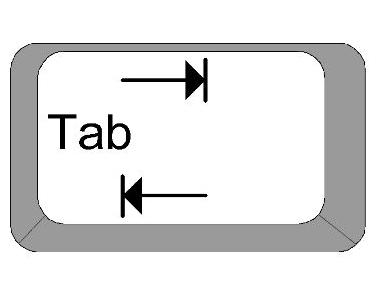
\includegraphics[scale=0.5]{../img/tab_key.jpg} para autocompletar las
  posibles rutas desde donde quiera que estes.
\item
  Escoge alguna (nuevamente usando la tecla tab para moverte entre las
  opciones). Si esto no funciona, teclea textualmente alguna de las
  rutas que ves.
\item
  Cierra la doble comilla y el paréntesis.
\item
  Teclea enter.
\item
  Debes encontrarte en la ruta elegida cuando tecleas \texttt{getwd()}.
\end{enumerate}

Con lo que acabamos de hacer, R buscará archivos o guardará archivos en
el folder \texttt{/home/animalito/study/}. En R también es posible
navegar a partir de el directorio de trabajo. Como siempre,

\begin{itemize}
\tightlist
\item
  ``../un\_archivo.R'' le indica a R que busque un folder arriba del
  actual directorio de trabajo por el archivo \emph{un\_archivo.R}.
\item
  ``datos/otro\_archivo.R'' hace que se busque en el directorio de
  trabajo, dentro del folder \emph{datos} por el archivo
  \emph{otro\_archivo.R}
\end{itemize}

\begin{nota}
\textbf{Rutas relativas vs. Rutas absolutas\\}

El resultado que se muestra aquí al usar el comando \texttt{getwd()} depende de la computadora en la que se esta 
trabajando debido a que es una \textit{ruta absoluta}. Nota como es diferente la ruta 
que obtienes al correr el comando en tu consola de \texttt{R}. Eso es porque se trata 
de una ruta absoluta, es decir, es tal que da la ruta (\textit{path}) completo
al directorio en cuestión. Puedes accesar todos los directorios o archivos usando su ruta absoluta.\\

En investigación reproducible (\textit{reproducible research}), en investigación colaborativa o
incluso cuando trabajas en varias computadoras es una buena idea usar rutas relativas
en lugar de absolutas. Esto hace que el código sea menos dependiente de una estructura
de archivos o computadora en particular \parencite[][p. 67]{gandrud2013}. \\

En general, es \textit{buena práctica} configurar el código de un proyecto con rutas relativas.
En \texttt{R} en particular, cuando guardas un \texttt{Rmarkdown} y lo corres desde la línea de
comandos (o lo \textit{tejes} desde \texttt{RStudio}), la ruta que está fija -como si hubieras usado el comando \texttt{setwd()} es
en donde \textit{vive} ese archivo, es decir, el directorio en donde está guardado el mismo.\\

Desde cualquier \texttt{script} puedes llamar a otros usando este tipo de ruta como en 
el ejemplo anterior.
\end{nota}

\subsection{Ejemplos básicos}\label{ejemplos-basicos}

La consola permite hacer operaciones sobre números o caracteres (cuando
tiene sentido).

\begin{Shaded}
\begin{Highlighting}[]
\CommentTok{# Potencias, sumas, multiplicaciones}
\DecValTok{2}\NormalTok{^}\DecValTok{3} \NormalTok{+}\StringTok{ }\DecValTok{67} \NormalTok{*}\StringTok{ }\DecValTok{4} \NormalTok{-}\StringTok{ }\NormalTok{(}\DecValTok{45} \NormalTok{+}\StringTok{ }\DecValTok{5}\NormalTok{)}
\end{Highlighting}
\end{Shaded}

\begin{verbatim}
## [1] 226
\end{verbatim}

\begin{Shaded}
\begin{Highlighting}[]
\CommentTok{# Comparaciones}
\DecValTok{56} \NormalTok{>}\StringTok{ }\DecValTok{78} 
\end{Highlighting}
\end{Shaded}

\begin{verbatim}
## [1] FALSE
\end{verbatim}

\begin{Shaded}
\begin{Highlighting}[]
\DecValTok{34} \NormalTok{<=}\StringTok{ }\DecValTok{34}
\end{Highlighting}
\end{Shaded}

\begin{verbatim}
## [1] TRUE
\end{verbatim}

\begin{Shaded}
\begin{Highlighting}[]
\DecValTok{234} \NormalTok{<}\StringTok{ }\DecValTok{345}
\end{Highlighting}
\end{Shaded}

\begin{verbatim}
## [1] TRUE
\end{verbatim}

\begin{Shaded}
\begin{Highlighting}[]
\StringTok{"hola"} \NormalTok{==}\StringTok{ "hola"}
\end{Highlighting}
\end{Shaded}

\begin{verbatim}
## [1] TRUE
\end{verbatim}

\begin{Shaded}
\begin{Highlighting}[]
\StringTok{"buu"} \NormalTok{!=}\StringTok{ "yay"}
\end{Highlighting}
\end{Shaded}

\begin{verbatim}
## [1] TRUE
\end{verbatim}

\begin{Shaded}
\begin{Highlighting}[]
\CommentTok{# módulo}
\DecValTok{10} \NormalTok\StringTok{ }\DecValTok{4} 
\end{Highlighting}
\end{Shaded}

\begin{verbatim}
## [1] 2
\end{verbatim}

Estas operaciones también pueden ser realizadas entre vectores\footnote{Revisaremos
  más adelante con detalle la definición de vectores en la sección
  \ref{estructuras-de-datos}.}.

\begin{Shaded}
\begin{Highlighting}[]
\CommentTok{# Creamos un vector con entradas del -1 al 12 y lo asignamos a la variable x}
\NormalTok{x <-}\StringTok{ }\NormalTok{-}\DecValTok{1}\NormalTok{:}\DecValTok{12}
\CommentTok{# Lo vemos}
\NormalTok{x}
\end{Highlighting}
\end{Shaded}

\begin{verbatim}
##  [1] -1  0  1  2  3  4  5  6  7  8  9 10 11 12
\end{verbatim}

\begin{Shaded}
\begin{Highlighting}[]
\CommentTok{# Le sumamos 1 a todas las entradas}
\NormalTok{x +}\StringTok{ }\DecValTok{1}
\end{Highlighting}
\end{Shaded}

\begin{verbatim}
##  [1]  0  1  2  3  4  5  6  7  8  9 10 11 12 13
\end{verbatim}

\begin{Shaded}
\begin{Highlighting}[]
\CommentTok{# Multiplicamos por 2 cada entrada y le sumamos 3}
\DecValTok{2} \NormalTok{*}\StringTok{ }\NormalTok{x +}\StringTok{ }\DecValTok{3}
\end{Highlighting}
\end{Shaded}

\begin{verbatim}
##  [1]  1  3  5  7  9 11 13 15 17 19 21 23 25 27
\end{verbatim}

\begin{Shaded}
\begin{Highlighting}[]
\CommentTok{# Sacamos el módulo de cada entrada}
\NormalTok{x %%}\StringTok{ }\DecValTok{5} 
\end{Highlighting}
\end{Shaded}

\begin{verbatim}
##  [1] 4 0 1 2 3 4 0 1 2 3 4 0 1 2
\end{verbatim}

\subsection{Comandos útiles}\label{comandos-utiles}

Para enlistar los objetos que están en el espacio de trabajo

\begin{Shaded}
\begin{Highlighting}[]
\KeywordTok{ls}\NormalTok{()}
\end{Highlighting}
\end{Shaded}

\begin{verbatim}
## [1] "x"
\end{verbatim}

Para eliminar todos los objetos en un workspace

\begin{Shaded}
\begin{Highlighting}[]
\KeywordTok{rm}\NormalTok{(}\DataTypeTok{list =} \KeywordTok{ls}\NormalTok{()) }\CommentTok{# se puede borrar solo uno, por ejemplo, nombrándolo}
\KeywordTok{ls}\NormalTok{()}
\end{Highlighting}
\end{Shaded}

\begin{verbatim}
## character(0)
\end{verbatim}

También se puede utilizar/guardar la historia de comandos utilizados

\begin{Shaded}
\begin{Highlighting}[]
\KeywordTok{history}\NormalTok{()}
\KeywordTok{history}\NormalTok{(}\DataTypeTok{max.show =} \DecValTok{5}\NormalTok{)}
\KeywordTok{history}\NormalTok{(}\DataTypeTok{max.show =} \OtherTok{Inf}\NormalTok{) }\CommentTok{# Muestra toda la historia}

\CommentTok{# Se puede salvar la historia de comandos a un archivo}
\KeywordTok{savehistory}\NormalTok{(}\DataTypeTok{file =} \StringTok{"mihistoria"}\NormalTok{) }\CommentTok{# Por default, R ya hace esto }
\CommentTok{# en un archivo ".Rhistory"}

\CommentTok{# Cargar al espacio de trabajo actual (current workspace) una }
\CommentTok{# historia de comandos en particular}
\KeywordTok{loadhistory}\NormalTok{(}\DataTypeTok{file =} \StringTok{"mihistoria"}\NormalTok{)}
\end{Highlighting}
\end{Shaded}

Es posible también guardar el workspace -en forma completa- en un
archivo con el comando \texttt{save.image()} a un archivo con extensión
\emph{.RData}. Puedes guardar una lista de objetos específica a un
archivo \emph{.RData}. Por ejemplo:

\begin{Shaded}
\begin{Highlighting}[]
\NormalTok{x <-}\StringTok{ }\DecValTok{1}\NormalTok{:}\DecValTok{12}
\NormalTok{y <-}\StringTok{ }\DecValTok{3}\NormalTok{:}\DecValTok{45}
\KeywordTok{save}\NormalTok{(x, y, }\DataTypeTok{file =} \StringTok{"ejemplo.RData"}\NormalTok{) }\CommentTok{#la extensión puede ser arbitraria.}
\end{Highlighting}
\end{Shaded}

Después puedo cargar ese archivo. Prueba hacer:

\begin{Shaded}
\begin{Highlighting}[]
\KeywordTok{rm}\NormalTok{(}\DataTypeTok{list =} \KeywordTok{ls}\NormalTok{()) }\CommentTok{# limpiamos workspace}
\KeywordTok{load}\NormalTok{(}\DataTypeTok{file =} \StringTok{"ejemplo.RData"}\NormalTok{) }\CommentTok{#la extensión puede ser arbitraria.}
\KeywordTok{ls}\NormalTok{()}
\end{Highlighting}
\end{Shaded}

Nota como los objetos preservan el nombre con el que fueron guardados.

\section{Librerías}\label{librerias}

R puede hacer muchos análisis estadísticos y de datos. Las diferentes
capacidades están organizadas en paquetes o librerías. Con la
\href{https://github.com/animalito/aprendeR/blob/master/lecture_01/0_instalacion.pdf}{instalación
estándar} se instalan también los paquetes más comunes. Para obtener una
lista de todos los paquetes instalados se puede utilizar el comando
\texttt{library()} en la consola o en un script.

Existen una gran cantidad de paquetes disponibles además de los
incluidos por omisión (\emph{default}).

\subsection{CRAN}\label{cran}

\emph{Comprehensive R Archive Network} {[}@cran{]} es una colección de
sitios que contienen exactamente el mismo material, es decir, son
espejos (\emph{mirrors}) de las distribuciones de R, las extensiones, la
documentación y los binarios. El master de CRAN está en
Wirtschaftsuniversität Wien en Austria. Éste se ``espeja''
(\emph{mirrors}) en forma diaria a muchos sitios alrededor del mundo. En
la \href{https://cran.r-project.org/mirrors.html}{lista de espejos} se
puede ver que para México están disponibles el espejo del ITAM, del
Colegio de Postgraduados (Texcoco) y Jellyfish Foundation {[}@cran{]}.

Los espejos son importantes pues, cada vez que busquen instalar
paquetes, se les preguntará qué espejo quieren utilizar para la sesión
en cuestión. Del espejo que selecciones, será del cuál R \emph{bajará}
el binario y la documentación.

Del CRAN es que se obtiene la última versión oficial de R. Diario se
actualizan los espejos. Para más detalles consultar el
\href{https://cran.r-project.org/doc/FAQ/R-FAQ.html}{FAQ}.

Para contribuir un paquete en CRAN se deben seguir las instrucciones
\href{https://cran.r-project.org/web/packages/policies.html}{aquí}.

\subsection{Github}\label{github}

Git es un controlador de versiones muy popular para desarrollar
software. Cuando se combina con \href{https://github.com/}{GitHub} se
puede compartir el código con el resto de la comunidad. Éste controlador
de versiones es el más popular entre los que contribuyen a R. Muchos
problemas a los que uno se enfrenta alguien ya los desarrolló y no
necesariamente publicó el paquete en CRAN. Para instalar algún paquete
desde GitHub, se pueden seguir las instrucciones siguientes

\begin{Shaded}
\begin{Highlighting}[]
\KeywordTok{install.packages}\NormalTok{(}\StringTok{"devtools"}\NormalTok{)}
\NormalTok{devtools::}\KeywordTok{install_github}\NormalTok{(}\StringTok{"username/packagename"}\NormalTok{)}
\end{Highlighting}
\end{Shaded}

Donde \texttt{username} es el usuario de Github y \texttt{packagename}
es el nombre del repositorio que contiene el paquete. Cuidado, no todo
repositorio en GitHub es un paquete. Para más información ver el
capítulo \href{http://r-pkgs.had.co.nz/git.html}{Git and GitHub} en
\textcite{wickham2015r}.

\subsection{Otras fuentes}\label{otras-fuentes}

Otros lugares en donde es común que se publiquen paquetes es en
\href{https://www.bioconductor.org/}{Bioconductor} un projecto de
software para la comprensión de datos del genoma humano.

\section{Paquetes recomendados}\label{paquetes-recomendados}

Hay muchísimas librerías y lo recomendable es, dado un problema y un
modelo para resolverlo, revisar si alguien ya implementó el método en
algunas de las fuentes de paquetes mencionadas antes.

Para mantener orden en los paquetes descargados puede ser útil utilizar
el \textcite{pacman} pues provee de herramientas para instalar paquetes
en una forma un poco más sencilla que usando la función
\texttt{install.packages}.

En particular, la función \texttt{p\_load} permite instalar, cargar y
actualizar uno o varios paquetes.

Si queremos instalar varios paquetes usando las herramientas del R
básico (\emph{base}) {[}@rbase{]} haríamos algo como
\parencite[ejemplo tomado de][en la viñeta de intrducción al paquete]{pacman}:

\begin{Shaded}
\begin{Highlighting}[]
\NormalTok{packs <-}\StringTok{ }\KeywordTok{c}\NormalTok{(}\StringTok{"XML"}\NormalTok{, }\StringTok{"devtools"}\NormalTok{, }\StringTok{"RCurl"}\NormalTok{, }\StringTok{"fakePackage"}\NormalTok{, }\StringTok{"SPSSemulate"}\NormalTok{)}
\NormalTok{success <-}\StringTok{ }\KeywordTok{suppressWarnings}\NormalTok{(}\KeywordTok{sapply}\NormalTok{(packs, require, }\DataTypeTok{character.only =} \OtherTok{TRUE}\NormalTok{))}
\KeywordTok{install.packages}\NormalTok{(}\KeywordTok{names}\NormalTok{(success)[!success])}
\KeywordTok{sapply}\NormalTok{(}\KeywordTok{names}\NormalTok{(success)[!success], require, }\DataTypeTok{character.only =} \OtherTok{TRUE}\NormalTok{)}
\end{Highlighting}
\end{Shaded}

Con \texttt{pacman::p\_load} la tarea se reduce a:

\begin{Shaded}
\begin{Highlighting}[]
\NormalTok{pacman::}\KeywordTok{p_load}\NormalTok{(XML, devtools, RCurl, fakePackage, SPSSemulate)}
\end{Highlighting}
\end{Shaded}

\begin{curiosidad}
Nota como se puede llamar a una función por su nombre \texttt{p\_load} una vez que 
ya cargamos el paquete en el cuál esa función está guardada con el comando \texttt{library(pacman)}
o podemos llamarla directamente utilizando la convención \texttt{paquete::funcion}, en este caso,
\texttt{pacman::p\_load}.
\end{curiosidad}

Para instalar \texttt{pacman} escribe:

\begin{Shaded}
\begin{Highlighting}[]
\KeywordTok{install.packages}\NormalTok{(}\StringTok{"pacman"}\NormalTok{)}
\end{Highlighting}
\end{Shaded}

Algunos paquetes se encuentran en desarrollo. En particular, si se
encuentran en \texttt{github} pueden descargarse usando la función
\texttt{pacman::p\_install\_gh(\textquotesingle{}usuario/repositorio\textquotesingle{})}.

A continuación, hay una lista de paquetes que se recomienda descargar
para tener a la mano herramientas diversas útiles para el trabajo del
científico de datos. La lista no es comprensiva pues hay un gran número
de paquetes útiles.

\begin{Shaded}
\begin{Highlighting}[]
\CommentTok{# Para cargar datos al ambiente de trabajo (data load)}
\NormalTok{pacman::}\KeywordTok{p_load}\NormalTok{(RODBC, RMySQL, RPostgreSQL, RSQLite, foreign, Rpostgres, haven}
               \NormalTok{, readr)}
\NormalTok{pacman::}\KeywordTok{p_install_gh}\NormalTok{(}\StringTok{"hadley/readxl"}\NormalTok{)}
\NormalTok{pacman::}\KeywordTok{p_install_gh}\NormalTok{(}\StringTok{"rstats-db/RPostgres"}\NormalTok{)}

\CommentTok{# Para manipular datos (data manipulation)}
\NormalTok{pacman::}\KeywordTok{p_load}\NormalTok{(plyr, dplyr, data.table, tidyr, stringr, lubridate, gsubfn)}

\CommentTok{# Para visualizar datos (data visualization)}
\NormalTok{pacman::}\KeywordTok{p_load}\NormalTok{(ggplot2, graphics, ggvis)}
\NormalTok{pacman::}\KeywordTok{p_install_gh}\NormalTok{(}\StringTok{"RcppCore/Rcpp"}\NormalTok{)}
\NormalTok{pacman::}\KeywordTok{p_install_gh}\NormalTok{(}\StringTok{"rstats-db/DBI"}\NormalTok{)}
\NormalTok{pacman::}\KeywordTok{p_install_gh}\NormalTok{(}\StringTok{'ramnathv/htmlwidgets'}\NormalTok{)}
\NormalTok{pacman::}\KeywordTok{p_install_gh}\NormalTok{(}\StringTok{'rstudio/leaflet'}\NormalTok{)}
\NormalTok{pacman::}\KeywordTok{p_install_gh}\NormalTok{(}\StringTok{'bwlewis/rthreejs'}\NormalTok{)}
\NormalTok{pacman::}\KeywordTok{p_install_gh}\NormalTok{(}\StringTok{'htmlwidgets/sparkline'}\NormalTok{)}
\NormalTok{pacman::}\KeywordTok{p_load}\NormalTok{(dygraphs, DT, DiagrammeR, networkD3, googleVis)}

\CommentTok{# Para modelar (data modelling)}
\NormalTok{pacman::}\KeywordTok{p_load}\NormalTok{(car, mgcv, lme4, nlme, randomForest, multcomp, vcd, glmnet, survival, caret)}

\CommentTok{# Para generar reportes (reports)}
\NormalTok{pacman::}\KeywordTok{p_load}\NormalTok{(shiny, xtable, knitr, rmarkdown)}

\CommentTok{# Para trabajar con datos espaciales (spatial data)}
\NormalTok{pacman::}\KeywordTok{p_load}\NormalTok{(sp, maptools, maps, ggmap, rgdal)}

\CommentTok{# Para trabajo con series de tiempo (time series)}
\NormalTok{pacman::}\KeywordTok{p_load}\NormalTok{(zoo, quantmod)}

\CommentTok{# Para escribir código de alto rendimiento en R (High performance R code)}
\NormalTok{pacman::}\KeywordTok{p_load}\NormalTok{(Rcpp, parallel)}

\CommentTok{# Trabajar con la web }
\NormalTok{pacman::}\KeywordTok{p_load}\NormalTok{(XML, jsonlite, httr)}

\CommentTok{# Para escribir paquetes en R}
\NormalTok{pacman::}\KeywordTok{p_load}\NormalTok{(devtools, testthat, roxygen2)}
\end{Highlighting}
\end{Shaded}

\section{Scripting}\label{scripting}

R es un intérprete. Utiliza un ambiente basado en línea de comandos. Por
ende, es necesario escribir la secuencia de comandos que se desea
realizar a diferencia de otras herramientas en donde es posible utlizar
el mouse o menús.

Aunque los comandos pueden ser ejecutados directamente en consola una
única vez, también es posible guardarlos en archivos conocidos como
\emph{scripts}. Típicamente, utilizamos la extensión \textbf{.R} o
\textbf{.r}. En RStudio, \texttt{CTRL\ +\ SHIFT\ +\ N} abre
inmediatamente un nuevo editor en el panel superior izquierdo.

Se puede \emph{ir editando} el script y corriendo los comandos línea por
línea con \texttt{CTRL\ +\ ENTER}. Esto también aplica para
\emph{correr} una selección del texto editable.

Es posible también correr todo el script

\begin{Shaded}
\begin{Highlighting}[]
\KeywordTok{source}\NormalTok{(}\StringTok{"foo.R"}\NormalTok{)}
\end{Highlighting}
\end{Shaded}

O con el atajo \texttt{CTRL\ +\ SHIFT\ +\ S} en RStudio.

Para enlistar algunos shortcuts comunes en RStudio presiona
\texttt{ALT\ +\ SHIFT\ +\ K}. De la misma manera, si utilizas Emacs +
ESS, existen múltiples atajos de teclado para realizar todo mucho más
eficientemente. Estudiarlos no es tiempo perdido.

\section{Ayuda y documentación}\label{ayuda-y-documentacion}

R tiene mucha documentación. Desde la consola se puede accesar a la
misma.

Para ayuda general,

\begin{Shaded}
\begin{Highlighting}[]
\KeywordTok{help.start}\NormalTok{()}
\end{Highlighting}
\end{Shaded}

Para la ayuda de una función en especifico, por ejemplo, si se quiere
graficar algo y sabemos que existe la funcion \texttt{plot} podemos
consultar fácilmente la ayuda.

\begin{Shaded}
\begin{Highlighting}[]
\KeywordTok{help}\NormalTok{(plot)}
\CommentTok{# o tecleando directamente}
\NormalTok{?plot}
\end{Highlighting}
\end{Shaded}

El segundo ejemplo se puede extender para buscar esa función en todos
los paquetes que tengo instalados en mi ambiente al escribir
\texttt{??plot}.

La documetnación normalmente se acompaña de ejemplos. Para \emph{correr}
los ejemplos sin necesidad de copiar y pegar, prueba

\begin{Shaded}
\begin{Highlighting}[]
\KeywordTok{example}\NormalTok{(plot)}
\end{Highlighting}
\end{Shaded}

Para búsquedas más comprensivas, se puede buscar de otras maneras:

\begin{Shaded}
\begin{Highlighting}[]
\KeywordTok{apropos}\NormalTok{(}\StringTok{"foo"}\NormalTok{) }\CommentTok{# Enlista todas las funciones que contengan la cadena "foo"}
\KeywordTok{RSiteSearch}\NormalTok{(}\StringTok{"foo"}\NormalTok{) }\CommentTok{# Busca por la cadena "foo" en todos los manuales de ayuda }
\CommentTok{# y listas de distribución.}
\end{Highlighting}
\end{Shaded}

\section{Estructuras de datos}\label{estructuras-de-datos}

R tiene diferentes tipos y estructuras de datos que permiten al usuario
aprovechar el lenguaje. La manipulación de estos objetos es algo que se
hace diario y entender cómo operarlos o cómo convertir de una a otra es
muy útil.

\renewcommand\bcStyleTitre[1]{\large\textcolor{ttblue}{#1}}

\begin{bclogo}[
  couleur=bgblue,
  arrondi=0,
  logo=\bcattention,
  barre=none,
  noborder=true]{En R}
\begin{itemize}
\item Todo lo que existe es un objeto.
\item Todo lo que sucede es una llamada a una función.
\end{itemize}
\end{bclogo}

\subsection{Clases atómicas (atomic
classes)}\label{clases-atomicas-atomic-classes}

R tiene 6 clases atómicas.

\begin{itemize}
\tightlist
\item
  character (\emph{caracter})
\item
  numeric (números reales o decimales)
\item
  integer (números enteros)
\item
  logical (booleanos, i.e.~falsos-verdaderos)
\item
  complex (números complejos)
\end{itemize}

\begin{table}[ht]
\centering
\begin{tabular}{p{3cm}p{5cm}}
  \hline
Tipo & Ejemplo \\ 
  \hline
Caracter & "hola", "x" \\ 
Numérico & 67, 45.5 \\
Integer & 2L, 67L \\
Lógico & TRUE, FALSE, T, F \\
Complejo & 1 + 4i\\
   \hline
\end{tabular}
\caption{Clases atómicas.}
\end{table}

Algunos comandos importantes para las clases atómicas son su tipo
\texttt{typeof()}, su tamaño \texttt{length()} y sus atributos
\texttt{attributes()}, es decir, sus metadatos.

\begin{Shaded}
\begin{Highlighting}[]
\NormalTok{############ Ejemplo 1}

\NormalTok{x <-}\StringTok{ "una cadena"}
\KeywordTok{typeof}\NormalTok{(x)}
\end{Highlighting}
\end{Shaded}

\begin{verbatim}
## [1] "character"
\end{verbatim}

\begin{Shaded}
\begin{Highlighting}[]
\KeywordTok{length}\NormalTok{(x) }\CommentTok{# tamaño: cuántas cadenas son?}
\end{Highlighting}
\end{Shaded}

\begin{verbatim}
## [1] 1
\end{verbatim}

\begin{Shaded}
\begin{Highlighting}[]
\KeywordTok{nchar}\NormalTok{(x) }\CommentTok{# Número de caracteres}
\end{Highlighting}
\end{Shaded}

\begin{verbatim}
## [1] 10
\end{verbatim}

\begin{Shaded}
\begin{Highlighting}[]
\KeywordTok{attributes}\NormalTok{(x) }\CommentTok{# Le pusimos metadatos?}
\end{Highlighting}
\end{Shaded}

\begin{verbatim}
## NULL
\end{verbatim}

\begin{Shaded}
\begin{Highlighting}[]
\NormalTok{############ Ejemplo 2}

\NormalTok{y <-}\StringTok{ }\DecValTok{1}\NormalTok{:}\DecValTok{10}
\KeywordTok{typeof}\NormalTok{(y)}
\end{Highlighting}
\end{Shaded}

\begin{verbatim}
## [1] "integer"
\end{verbatim}

\begin{Shaded}
\begin{Highlighting}[]
\KeywordTok{length}\NormalTok{(y)}
\end{Highlighting}
\end{Shaded}

\begin{verbatim}
## [1] 10
\end{verbatim}

\begin{Shaded}
\begin{Highlighting}[]
\KeywordTok{attributes}\NormalTok{(y)}
\end{Highlighting}
\end{Shaded}

\begin{verbatim}
## NULL
\end{verbatim}

\begin{Shaded}
\begin{Highlighting}[]
\NormalTok{############ Ejemplo 3}

\NormalTok{z <-}\StringTok{ }\KeywordTok{c}\NormalTok{(1L, 2L, 3L) }\CommentTok{# Nota como para denotar enteros debes incluir una L al final}
\KeywordTok{typeof}\NormalTok{(z)}
\end{Highlighting}
\end{Shaded}

\begin{verbatim}
## [1] "integer"
\end{verbatim}

\begin{Shaded}
\begin{Highlighting}[]
\KeywordTok{length}\NormalTok{(z)}
\end{Highlighting}
\end{Shaded}

\begin{verbatim}
## [1] 3
\end{verbatim}

\subsection{Vectores}\label{vectores}

Los vectores son la estructura de datos más común y básica de R. Hay dos
tipos de vectores: vectores atómicos y listas.

Típicamente -en libros, blogs, manuales, cuando se mencionan vectores se
refieren a los atómicos y no a las listas.

\subsubsection{Vectores atómicos}\label{vectores-atomicos}

Un vector es un conjunto de elementos con alguna de las clases atómicas,
es decir, \texttt{character}, \texttt{logical}, \texttt{integer},
\texttt{numeric}. Se puede crear un vector vacío con el comando
\texttt{vector()} así como especificar su tamaño y su clase.

\begin{Shaded}
\begin{Highlighting}[]
\NormalTok{v <-}\StringTok{ }\KeywordTok{vector}\NormalTok{()}
\NormalTok{v }
\end{Highlighting}
\end{Shaded}

\begin{verbatim}
## logical(0)
\end{verbatim}

\begin{Shaded}
\begin{Highlighting}[]
\NormalTok{## Especifico clase y longitud}
\KeywordTok{vector}\NormalTok{(}\StringTok{"character"}\NormalTok{, }\DataTypeTok{length =} \DecValTok{10}\NormalTok{)}
\end{Highlighting}
\end{Shaded}

\begin{verbatim}
##  [1] "" "" "" "" "" "" "" "" "" ""
\end{verbatim}

\begin{Shaded}
\begin{Highlighting}[]
\NormalTok{## Lo mismo pero usando un wrapper}
\KeywordTok{character}\NormalTok{(}\DecValTok{10}\NormalTok{)}
\end{Highlighting}
\end{Shaded}

\begin{verbatim}
##  [1] "" "" "" "" "" "" "" "" "" ""
\end{verbatim}

\begin{Shaded}
\begin{Highlighting}[]
\NormalTok{## Numerico de tamaño 5}
\KeywordTok{numeric}\NormalTok{(}\DecValTok{5}\NormalTok{)}
\end{Highlighting}
\end{Shaded}

\begin{verbatim}
## [1] 0 0 0 0 0
\end{verbatim}

\begin{Shaded}
\begin{Highlighting}[]
\NormalTok{## Lógico tamaño 5}
\KeywordTok{logical}\NormalTok{(}\DecValTok{5}\NormalTok{)}
\end{Highlighting}
\end{Shaded}

\begin{verbatim}
## [1] FALSE FALSE FALSE FALSE FALSE
\end{verbatim}

Realiza los siguientes ejemplos en la consola de R.

\begin{Shaded}
\begin{Highlighting}[]
\NormalTok{x <-}\StringTok{ }\KeywordTok{rep}\NormalTok{(}\DecValTok{1}\NormalTok{, }\DecValTok{5}\NormalTok{)}
\NormalTok{x}
\KeywordTok{typeof}\NormalTok{(x)}

\NormalTok{xi <-}\StringTok{ }\KeywordTok{c}\NormalTok{(1L, 3L, 56L, 4L)}
\NormalTok{xi}
\KeywordTok{typeof}\NormalTok{(xi)}

\NormalTok{y <-}\StringTok{ }\KeywordTok{c}\NormalTok{(T, F, T, F, F, T)}

\NormalTok{z <-}\StringTok{ }\KeywordTok{c}\NormalTok{(}\StringTok{"a"}\NormalTok{, }\StringTok{"aba"}\NormalTok{, }\StringTok{"andrea"}\NormalTok{, }\StringTok{"b"}\NormalTok{, }\StringTok{"bueno"}\NormalTok{)}
\KeywordTok{class}\NormalTok{(z)}
\KeywordTok{str}\NormalTok{(z)}
\end{Highlighting}
\end{Shaded}

\textbf{Operaciones con vectores}

Accesar partes del vector.

\begin{Shaded}
\begin{Highlighting}[]
\NormalTok{a <-}\StringTok{ }\KeywordTok{c}\NormalTok{(}\DecValTok{1}\NormalTok{:}\DecValTok{5}\NormalTok{)}
\NormalTok{a}
\end{Highlighting}
\end{Shaded}

\begin{verbatim}
## [1] 1 2 3 4 5
\end{verbatim}

\begin{Shaded}
\begin{Highlighting}[]
\NormalTok{a[}\DecValTok{1}\NormalTok{]}
\end{Highlighting}
\end{Shaded}

\begin{verbatim}
## [1] 1
\end{verbatim}

\begin{Shaded}
\begin{Highlighting}[]
\NormalTok{a[}\DecValTok{2}\NormalTok{]}
\end{Highlighting}
\end{Shaded}

\begin{verbatim}
## [1] 2
\end{verbatim}

\begin{Shaded}
\begin{Highlighting}[]
\NormalTok{a[}\DecValTok{4}\NormalTok{:}\DecValTok{5}\NormalTok{]}
\end{Highlighting}
\end{Shaded}

\begin{verbatim}
## [1] 4 5
\end{verbatim}

Aritmética: por default, se realizan componente a componente.

\begin{Shaded}
\begin{Highlighting}[]
\NormalTok{b <-}\StringTok{ }\NormalTok{a +}\StringTok{ }\DecValTok{10}
\NormalTok{b}
\end{Highlighting}
\end{Shaded}

\begin{verbatim}
## [1] 11 12 13 14 15
\end{verbatim}

\begin{Shaded}
\begin{Highlighting}[]
\NormalTok{c <-}\StringTok{ }\KeywordTok{sqrt}\NormalTok{(b) }\CommentTok{# square root = raíz}
\NormalTok{c}
\end{Highlighting}
\end{Shaded}

\begin{verbatim}
## [1] 3.316625 3.464102 3.605551 3.741657 3.872983
\end{verbatim}

\begin{Shaded}
\begin{Highlighting}[]
\NormalTok{a +}\StringTok{ }\NormalTok{c}
\end{Highlighting}
\end{Shaded}

\begin{verbatim}
## [1] 4.316625 5.464102 6.605551 7.741657 8.872983
\end{verbatim}

\begin{Shaded}
\begin{Highlighting}[]
\DecValTok{10} \NormalTok{*}\StringTok{ }\NormalTok{(a +}\StringTok{ }\NormalTok{c)}
\end{Highlighting}
\end{Shaded}

\begin{verbatim}
## [1] 43.16625 54.64102 66.05551 77.41657 88.72983
\end{verbatim}

\begin{Shaded}
\begin{Highlighting}[]
\NormalTok{a^}\DecValTok{2}
\end{Highlighting}
\end{Shaded}

\begin{verbatim}
## [1]  1  4  9 16 25
\end{verbatim}

\begin{Shaded}
\begin{Highlighting}[]
\NormalTok{a *}\StringTok{ }\NormalTok{c}
\end{Highlighting}
\end{Shaded}

\begin{verbatim}
## [1]  3.316625  6.928203 10.816654 14.966630 19.364917
\end{verbatim}

Agregar elementos aun vector ya creado

\begin{Shaded}
\begin{Highlighting}[]
\NormalTok{a <-}\StringTok{ }\KeywordTok{c}\NormalTok{(a, }\DecValTok{7}\NormalTok{)}
\NormalTok{a}
\end{Highlighting}
\end{Shaded}

\begin{verbatim}
## [1] 1 2 3 4 5 7
\end{verbatim}

Para construir datos rápido, podemos usar comandos como \texttt{rep},
\texttt{seq} o distintas distribuciones, e.g., la normal \texttt{rnorm},
uniformes \texttt{runif} o cualquiera en
\href{https://stat.ethz.ch/R-manual/R-devel/library/stats/html/Distributions.html}{esta
lista}.

Prueba lo siguiente:

\begin{Shaded}
\begin{Highlighting}[]
\CommentTok{# Dame un vector donde el minimo sea 0, maximo 1 en intervalos de 0.25}
\KeywordTok{seq}\NormalTok{(}\DecValTok{0}\NormalTok{, }\DecValTok{1}\NormalTok{, }\FloatTok{0.25}\NormalTok{)}
\CommentTok{# Vector con 10 unos}
\KeywordTok{rep}\NormalTok{(}\DecValTok{1}\NormalTok{, }\DecValTok{10}\NormalTok{)}
\CommentTok{# 5 realizaciones de una normal(0,1)}
\KeywordTok{rnorm}\NormalTok{(}\DecValTok{5}\NormalTok{)}
\CommentTok{# De una normal(10, 5)}
\KeywordTok{rnorm}\NormalTok{(}\DecValTok{5}\NormalTok{, }\DataTypeTok{mean =} \DecValTok{10}\NormalTok{, }\DataTypeTok{sd =} \KeywordTok{sqrt}\NormalTok{(}\DecValTok{5}\NormalTok{))}
\CommentTok{# De una uniforme(0,1)}
\KeywordTok{runif}\NormalTok{(}\DecValTok{5}\NormalTok{)}
\CommentTok{# De una uniforme(5, 15)}
\KeywordTok{runif}\NormalTok{(}\DecValTok{5}\NormalTok{, }\DataTypeTok{min =} \DecValTok{5}\NormalTok{, }\DataTypeTok{max =} \DecValTok{15}\NormalTok{)}
\end{Highlighting}
\end{Shaded}

\paragraph{Otros objetos importantes}\label{otros-objetos-importantes}

\texttt{Inf} es como R denomina al infinito. En el mundo de R se permite
también positivo o negativo.

\begin{Shaded}
\begin{Highlighting}[]
\DecValTok{1}\NormalTok{/}\DecValTok{0}
\end{Highlighting}
\end{Shaded}

\begin{verbatim}
## [1] Inf
\end{verbatim}

\begin{Shaded}
\begin{Highlighting}[]
\DecValTok{1}\NormalTok{/}\OtherTok{Inf}
\end{Highlighting}
\end{Shaded}

\begin{verbatim}
## [1] 0
\end{verbatim}

\texttt{NaN} es como R denota a algo que no es un número (literal:
\emph{not a number}).

\begin{Shaded}
\begin{Highlighting}[]
\DecValTok{0}\NormalTok{/}\DecValTok{0}
\end{Highlighting}
\end{Shaded}

\begin{verbatim}
## [1] NaN
\end{verbatim}

Cada objeto tiene atributos. Hay atributos específicos para vectores
que, sin importar su clase, tienen en común. Ya revisamos algunos:
tamaño (\texttt{length}), clase (\texttt{class}). También son
importantes atributos como los nombres

\begin{Shaded}
\begin{Highlighting}[]
\NormalTok{calificaciones <-}\StringTok{ }\KeywordTok{c}\NormalTok{(}\DecValTok{6}\NormalTok{, }\DecValTok{5}\NormalTok{, }\DecValTok{8}\NormalTok{, }\DecValTok{9}\NormalTok{, }\DecValTok{10}\NormalTok{)}
\KeywordTok{names}\NormalTok{(calificaciones) <-}\StringTok{ }\KeywordTok{c}\NormalTok{(}\StringTok{"Maria"}\NormalTok{, }\StringTok{"Jorge"}\NormalTok{, }\StringTok{"Miguel"}\NormalTok{, }\StringTok{"Raúl"}\NormalTok{, }\StringTok{"Carla"}\NormalTok{)}
\KeywordTok{attributes}\NormalTok{(calificaciones)}
\end{Highlighting}
\end{Shaded}

\begin{verbatim}
## $names
## [1] "Maria"  "Jorge"  "Miguel" "Raúl"   "Carla"
\end{verbatim}

\begin{Shaded}
\begin{Highlighting}[]
\CommentTok{# O llamamos directo a los nombres}
\KeywordTok{names}\NormalTok{(calificaciones)}
\end{Highlighting}
\end{Shaded}

\begin{verbatim}
## [1] "Maria"  "Jorge"  "Miguel" "Raúl"   "Carla"
\end{verbatim}

Mezclar tipos no es una buena idea

\begin{Shaded}
\begin{Highlighting}[]
\KeywordTok{c}\NormalTok{(}\FloatTok{1.7}\NormalTok{, }\StringTok{"a"}\NormalTok{)}
\end{Highlighting}
\end{Shaded}

\begin{verbatim}
## [1] "1.7" "a"
\end{verbatim}

\begin{Shaded}
\begin{Highlighting}[]
\KeywordTok{c}\NormalTok{(}\OtherTok{TRUE}\NormalTok{, }\DecValTok{2}\NormalTok{)}
\end{Highlighting}
\end{Shaded}

\begin{verbatim}
## [1] 1 2
\end{verbatim}

\begin{Shaded}
\begin{Highlighting}[]
\KeywordTok{c}\NormalTok{(}\StringTok{"a"}\NormalTok{, }\OtherTok{TRUE}\NormalTok{)}
\end{Highlighting}
\end{Shaded}

\begin{verbatim}
## [1] "a"    "TRUE"
\end{verbatim}

R realiza una coerción implícita entre los objetos y ``decide'' cuál es
la clase del vector. También hay coercioń explícita (\emph{explicit
coercion}) utilizando
\texttt{as.\textless{}nombre\_clase\textgreater{}}.

\begin{Shaded}
\begin{Highlighting}[]
\KeywordTok{as.numeric}\NormalTok{()}
\KeywordTok{as.character}\NormalTok{()}
\KeywordTok{as.integer}\NormalTok{()}
\KeywordTok{as.logical}\NormalTok{()}
\end{Highlighting}
\end{Shaded}

Muchos problemas suceden cuando le permites a R decidir por ti (o cuando
no sabes cuál decisión tomará R por \emph{default}).

\begin{Shaded}
\begin{Highlighting}[]
\NormalTok{x <-}\StringTok{ }\DecValTok{0}\NormalTok{:}\DecValTok{5}

\KeywordTok{identical}\NormalTok{(x, }\KeywordTok{as.numeric}\NormalTok{(x))}
\end{Highlighting}
\end{Shaded}

\begin{verbatim}
## [1] FALSE
\end{verbatim}

En este ejemplo, cuando declaramos \(x\) no especificamos su clase y R
decidió que era entero. Al coercionar al objeto para que fuese numérico,
R no considera a los dos objetos iguales. R te protege -no te permite
hacer o te advierte- de algunas cosas

\begin{Shaded}
\begin{Highlighting}[]
\DecValTok{1} \NormalTok{<}\StringTok{ "2"}
\end{Highlighting}
\end{Shaded}

\begin{verbatim}
## [1] TRUE
\end{verbatim}

Pero en otras, hace lo mejor que puede con lo que le das (cosa que a
veces no tiene sentido)

\begin{Shaded}
\begin{Highlighting}[]
\NormalTok{x <-}\StringTok{ }\KeywordTok{c}\NormalTok{(}\StringTok{"a"}\NormalTok{, }\StringTok{"b"}\NormalTok{, }\StringTok{"c"}\NormalTok{)}
\KeywordTok{as.numeric}\NormalTok{(x)}
\end{Highlighting}
\end{Shaded}

\begin{verbatim}
## [1] NA NA NA
\end{verbatim}

\begin{Shaded}
\begin{Highlighting}[]
\KeywordTok{as.logical}\NormalTok{(x)}
\end{Highlighting}
\end{Shaded}

\begin{verbatim}
## [1] NA NA NA
\end{verbatim}

\subsubsection{Matrices}\label{matrices}

Las matrices son un tipo especial de vectores. Son un vector atómico con
dimensión pues tienen filas y columnas.

\begin{Shaded}
\begin{Highlighting}[]
\NormalTok{m <-}\StringTok{ }\KeywordTok{matrix}\NormalTok{(}\KeywordTok{c}\NormalTok{(}\DecValTok{1}\NormalTok{, }\DecValTok{2}\NormalTok{, }\DecValTok{3}\NormalTok{, }\DecValTok{4}\NormalTok{), }\DataTypeTok{nrow =} \DecValTok{2}\NormalTok{, }\DataTypeTok{ncol =} \DecValTok{2}\NormalTok{)}
\NormalTok{m}
\end{Highlighting}
\end{Shaded}

\begin{verbatim}
##      [,1] [,2]
## [1,]    1    3
## [2,]    2    4
\end{verbatim}

Como puedes notar, las matrices se llenan siguiendo las columnas.
Podemos simplemente ``agregarle'' una dimensión a un vector para
construir una matriz.

\begin{Shaded}
\begin{Highlighting}[]
\NormalTok{m <-}\StringTok{ }\DecValTok{1}\NormalTok{:}\DecValTok{10}
\NormalTok{m}
\end{Highlighting}
\end{Shaded}

\begin{verbatim}
##  [1]  1  2  3  4  5  6  7  8  9 10
\end{verbatim}

\begin{Shaded}
\begin{Highlighting}[]
\KeywordTok{dim}\NormalTok{(m) <-}\StringTok{ }\KeywordTok{c}\NormalTok{(}\DecValTok{2}\NormalTok{, }\DecValTok{5}\NormalTok{)}
\NormalTok{m}
\end{Highlighting}
\end{Shaded}

\begin{verbatim}
##      [,1] [,2] [,3] [,4] [,5]
## [1,]    1    3    5    7    9
## [2,]    2    4    6    8   10
\end{verbatim}

También podemos pegar vectores de la misma longitud como si fueran
columnas de una matriz \texttt{cbind} o como si fueran filas
\texttt{rbind} (r = row, c = column).

\begin{Shaded}
\begin{Highlighting}[]
\NormalTok{x <-}\StringTok{ }\KeywordTok{runif}\NormalTok{(}\DecValTok{4}\NormalTok{)}
\NormalTok{y <-}\StringTok{ }\KeywordTok{rnorm}\NormalTok{(}\DecValTok{4}\NormalTok{)}
\KeywordTok{cbind}\NormalTok{(x, y)}
\end{Highlighting}
\end{Shaded}

\begin{verbatim}
##               x          y
## [1,] 0.18681273 -1.1640959
## [2,] 0.02267067 -2.3134259
## [3,] 0.91348432  0.3100017
## [4,] 0.99191958  0.2299862
\end{verbatim}

\begin{Shaded}
\begin{Highlighting}[]
\KeywordTok{rbind}\NormalTok{(x, y)}
\end{Highlighting}
\end{Shaded}

\begin{verbatim}
##         [,1]        [,2]      [,3]      [,4]
## x  0.1868127  0.02267067 0.9134843 0.9919196
## y -1.1640959 -2.31342586 0.3100017 0.2299862
\end{verbatim}

Le agregamos atributos para accesar más fácilmente a los objetos.

\begin{Shaded}
\begin{Highlighting}[]
\NormalTok{m <-}\StringTok{ }\KeywordTok{matrix}\NormalTok{(}\KeywordTok{c}\NormalTok{(x, y), }\DataTypeTok{nrow =} \DecValTok{4}\NormalTok{, }\DataTypeTok{ncol =} \DecValTok{2}\NormalTok{, }\DataTypeTok{byrow =} \NormalTok{T,}
            \DataTypeTok{dimnames =} \KeywordTok{list}\NormalTok{(}\KeywordTok{paste0}\NormalTok{(}\StringTok{"row"}\NormalTok{, }\DecValTok{1}\NormalTok{:}\DecValTok{4}\NormalTok{),}
                            \KeywordTok{paste0}\NormalTok{(}\StringTok{"col"}\NormalTok{, }\DecValTok{1}\NormalTok{:}\DecValTok{2}\NormalTok{)))}
\NormalTok{m}
\end{Highlighting}
\end{Shaded}

\begin{verbatim}
##            col1        col2
## row1  0.1868127  0.02267067
## row2  0.9134843  0.99191958
## row3 -1.1640959 -2.31342586
## row4  0.3100017  0.22998623
\end{verbatim}

\begin{Shaded}
\begin{Highlighting}[]
\NormalTok{m[}\DecValTok{1}\NormalTok{, }\DecValTok{1}\NormalTok{] ==}\StringTok{ }\NormalTok{m[}\StringTok{"row1"}\NormalTok{, }\StringTok{"col1"}\NormalTok{]}
\end{Highlighting}
\end{Shaded}

\begin{verbatim}
## [1] TRUE
\end{verbatim}

\begin{Shaded}
\begin{Highlighting}[]
\KeywordTok{dimnames}\NormalTok{(m)}
\end{Highlighting}
\end{Shaded}

\begin{verbatim}
## [[1]]
## [1] "row1" "row2" "row3" "row4"
## 
## [[2]]
## [1] "col1" "col2"
\end{verbatim}

\subsubsection{Listas}\label{listas}

Es un tipo de vector en el cuál cada elemento puede ser de un tipo
distinto. Mas aun, es posible incluir una lista como un elemento de otra
lista y por eso también se les conoce como vectores recursivos
(\emph{recursive vectors}).

Para crear una lista vacía utilizas \texttt{list()} y para coercionar un
objeto a una lista usa \texttt{as.list()}.

\begin{Shaded}
\begin{Highlighting}[]
\NormalTok{x <-}\StringTok{ }\KeywordTok{list}\NormalTok{(3L, }\FloatTok{3.56}\NormalTok{, }\DecValTok{1} \NormalTok{+}\StringTok{ }\NormalTok{4i, }\OtherTok{TRUE}\NormalTok{, }\StringTok{"hola"}\NormalTok{, }\KeywordTok{list}\NormalTok{(}\StringTok{"genial"}\NormalTok{, }\DecValTok{1}\NormalTok{))}
\NormalTok{x}
\end{Highlighting}
\end{Shaded}

\begin{verbatim}
## [[1]]
## [1] 3
## 
## [[2]]
## [1] 3.56
## 
## [[3]]
## [1] 1+4i
## 
## [[4]]
## [1] TRUE
## 
## [[5]]
## [1] "hola"
## 
## [[6]]
## [[6]][[1]]
## [1] "genial"
## 
## [[6]][[2]]
## [1] 1
\end{verbatim}

\begin{Shaded}
\begin{Highlighting}[]
\KeywordTok{length}\NormalTok{(x)}
\end{Highlighting}
\end{Shaded}

\begin{verbatim}
## [1] 6
\end{verbatim}

\begin{Shaded}
\begin{Highlighting}[]
\KeywordTok{class}\NormalTok{(x)}
\end{Highlighting}
\end{Shaded}

\begin{verbatim}
## [1] "list"
\end{verbatim}

\begin{Shaded}
\begin{Highlighting}[]
\KeywordTok{class}\NormalTok{(x[}\DecValTok{1}\NormalTok{])}
\end{Highlighting}
\end{Shaded}

\begin{verbatim}
## [1] "list"
\end{verbatim}

\begin{Shaded}
\begin{Highlighting}[]
\KeywordTok{class}\NormalTok{(x[[}\DecValTok{1}\NormalTok{]])}
\end{Highlighting}
\end{Shaded}

\begin{verbatim}
## [1] "integer"
\end{verbatim}

\begin{Shaded}
\begin{Highlighting}[]
\NormalTok{y <-}\StringTok{ }\KeywordTok{as.list}\NormalTok{(}\DecValTok{1}\NormalTok{:}\DecValTok{10}\NormalTok{)}
\KeywordTok{length}\NormalTok{(y)}
\end{Highlighting}
\end{Shaded}

\begin{verbatim}
## [1] 10
\end{verbatim}

Nota como muchas propiedades que tenían los vectores atómicos los tienen
también las listas. Por su propiedad recursiva, se navega diferente. Si
pides \texttt{x{[}1{]}} te devuelve una lista con lo que hayas puesto en
ese contenedor.

Para extraer el objeto (con la clase de ese objeto y no simplemente otra
lista) necesitas usar \texttt{x{[}{[}1{]}{]}}, es decir, el integer 3.

Las listas también pueden tener nombres

\begin{Shaded}
\begin{Highlighting}[]
\CommentTok{# Lista vacia}
\NormalTok{lista <-}\StringTok{ }\KeywordTok{list}\NormalTok{()}
\NormalTok{lista[[}\StringTok{"numeros"}\NormalTok{]] <-}\StringTok{ }\KeywordTok{c}\NormalTok{(}\DecValTok{1}\NormalTok{, }\DecValTok{34}\NormalTok{, }\FloatTok{45.5}\NormalTok{, }\DecValTok{34}\NormalTok{) }
\NormalTok{lista[[}\StringTok{"datos"}\NormalTok{]] <-}\StringTok{ }\KeywordTok{head}\NormalTok{(iris)}

\NormalTok{lista}
\end{Highlighting}
\end{Shaded}

\begin{verbatim}
## $numeros
## [1]  1.0 34.0 45.5 34.0
## 
## $datos
##   Sepal.Length Sepal.Width Petal.Length Petal.Width Species
## 1          5.1         3.5          1.4         0.2  setosa
## 2          4.9         3.0          1.4         0.2  setosa
## 3          4.7         3.2          1.3         0.2  setosa
## 4          4.6         3.1          1.5         0.2  setosa
## 5          5.0         3.6          1.4         0.2  setosa
## 6          5.4         3.9          1.7         0.4  setosa
\end{verbatim}

\begin{curiosidad}
R tiene muchos \href{https://stat.ethz.ch/R-manual/R-devel/library/datasets/html/00Index.html}{datos de ejemplo}
que son utilizados en muchos paquetes, blogs y libros. Utiliza {\bf help(iris)} para
saber más del dataset usado arriba.
\end{curiosidad}

\subsubsection{Factores (factor)}\label{factores-factor}

Otro tipo de vector pero que ayuda a representar datos del tipo
categórico u ordinal. Es muy importante decirle a R que algo debe ser
tratado como factor cuando se empieza a modelar o incluso para que los
métodos de gráficos funcionen de manera apropiada. Sin embargo, hay que
entender bien cómo tratarlos porque mal usados hacen que pasen muchas
cosas muy raras que dan resultados que estan \emph{mal, mal, mal}.

Los factores son enteros pero con etiquetas encima.

\begin{Shaded}
\begin{Highlighting}[]
\NormalTok{x <-}\StringTok{ }\KeywordTok{factor}\NormalTok{(}\KeywordTok{c}\NormalTok{(}\StringTok{"no"}\NormalTok{, }\StringTok{"si"}\NormalTok{, }\StringTok{"si"}\NormalTok{, }\StringTok{"no"}\NormalTok{))}
\NormalTok{x}
\end{Highlighting}
\end{Shaded}

\begin{verbatim}
## [1] no si si no
## Levels: no si
\end{verbatim}

Lo que te deja utilizar métodos para factores como tablas de frecuencias

\begin{Shaded}
\begin{Highlighting}[]
\KeywordTok{table}\NormalTok{(x)}
\end{Highlighting}
\end{Shaded}

\begin{verbatim}
## x
## no si 
##  2  2
\end{verbatim}

Los factores se van a ver \emph{como si fueran} vectores tipo caracter.
A veces se comportan como character vectors pero \emph{debemos} recordar
que por abajo son integers y tenemos que ser cuidadosos si los tratamos
como caracteres. Algunos métodos que están hechos para caracteres
coersionan un factor a caracter mientras que otros arrojan un error. Si
usas métodos de caracteres, lo mejor es ``castear'' a caracter tu factor
\texttt{as.character(mifactor)}. Pierdes algunas cosas pero te aseguras
que las cosas funcionen como deben.

\begin{Shaded}
\begin{Highlighting}[]
\KeywordTok{summary}\NormalTok{(x)}
\end{Highlighting}
\end{Shaded}

\begin{verbatim}
## no si 
##  2  2
\end{verbatim}

\begin{Shaded}
\begin{Highlighting}[]
\KeywordTok{summary}\NormalTok{(}\KeywordTok{as.character}\NormalTok{(x))}
\end{Highlighting}
\end{Shaded}

\begin{verbatim}
##    Length     Class      Mode 
##         4 character character
\end{verbatim}

Los factores pueden contener únicamente valores predefinidos. Por eso la
``unión'' de factores puede tronar.

\begin{Shaded}
\begin{Highlighting}[]
\NormalTok{y <-}\StringTok{ }\KeywordTok{factor}\NormalTok{(}\KeywordTok{c}\NormalTok{(}\StringTok{"si"}\NormalTok{, }\StringTok{"no"}\NormalTok{, }\StringTok{"tal vez"}\NormalTok{))}
\KeywordTok{c}\NormalTok{(x, y)}
\end{Highlighting}
\end{Shaded}

\begin{verbatim}
## [1] 1 2 2 1 2 1 3
\end{verbatim}

\begin{Shaded}
\begin{Highlighting}[]
\KeywordTok{class}\NormalTok{(}\KeywordTok{c}\NormalTok{(x, y))}
\end{Highlighting}
\end{Shaded}

\begin{verbatim}
## [1] "integer"
\end{verbatim}

¿Cómo recuperas el valor de las etiquetas? R hizo lo que pudo y está
mal. Para hacerlo bien, debemos

\begin{Shaded}
\begin{Highlighting}[]
\KeywordTok{factor}\NormalTok{(}\KeywordTok{c}\NormalTok{(}\KeywordTok{as.character}\NormalTok{(x), }\KeywordTok{as.character}\NormalTok{(y)))}
\end{Highlighting}
\end{Shaded}

\begin{verbatim}
## [1] no      si      si      no      si      no      tal vez
## Levels: no si tal vez
\end{verbatim}

Para datos ordinales como las respuestas en una pregunta de encuesta con
escala likert, podemos usar

\begin{Shaded}
\begin{Highlighting}[]
\KeywordTok{set.seed}\NormalTok{(}\DecValTok{2887}\NormalTok{)}
\NormalTok{respuestas <-}\StringTok{ }\KeywordTok{sample}\NormalTok{(}\DataTypeTok{x =} \KeywordTok{c}\NormalTok{(}\DecValTok{1}\NormalTok{:}\DecValTok{5}\NormalTok{), }\DataTypeTok{size =} \DecValTok{5}\NormalTok{, }\DataTypeTok{replace =}  \NormalTok{T)}
\NormalTok{respuestas }
\end{Highlighting}
\end{Shaded}

\begin{verbatim}
## [1] 4 1 4 2 1
\end{verbatim}

\begin{Shaded}
\begin{Highlighting}[]
\NormalTok{y <-}\StringTok{ }\KeywordTok{factor}\NormalTok{(}
  \DataTypeTok{x =} \NormalTok{respuestas,}
  \DataTypeTok{levels =} \KeywordTok{c}\NormalTok{(}\StringTok{"1"}\NormalTok{, }\StringTok{"2"}\NormalTok{, }\StringTok{"3"}\NormalTok{, }\StringTok{"4"}\NormalTok{, }\StringTok{"5"}\NormalTok{),}
  \DataTypeTok{labels =} \KeywordTok{c}\NormalTok{(}\StringTok{"muy en contra"}\NormalTok{, }\StringTok{"en contra"}\NormalTok{, }\StringTok{"indiferente"}\NormalTok{, }\StringTok{"a favor"}\NormalTok{, }\StringTok{"muy a favor"}\NormalTok{),}
  \DataTypeTok{ordered =} \NormalTok{T)}
\NormalTok{y}
\end{Highlighting}
\end{Shaded}

\begin{verbatim}
## [1] a favor       muy en contra a favor       en contra     muy en contra
## 5 Levels: muy en contra < en contra < indiferente < ... < muy a favor
\end{verbatim}

Nota como aunque no tengamos todos las respuestas, nuestro factor sabe
que las no ocurrencias son factibles (los niveles y las etiquetas las
incluyen).

\begin{Shaded}
\begin{Highlighting}[]
\KeywordTok{table}\NormalTok{(y)}
\end{Highlighting}
\end{Shaded}

\begin{verbatim}
## y
## muy en contra     en contra   indiferente       a favor   muy a favor 
##             2             1             0             2             0
\end{verbatim}

\begin{nota}[Nota]
En R muchas cosas se reducen a utlizar la estructura de datos apropiada y darle
todos los metadatos necesarios al objeto para que R no haga tonterias.
\end{nota}

\subsection{Data frames}\label{data-frames}

Los dataframes son uno de los objetos más importantes en R. Tanto así
que muchos no dejarían R porque implica abandonar este objeto. En
python, se intenta replicar este objeto con la librería \texttt{pandas}.

Este objeto es tan importante porque muchos de los modelos estadísticos
que se utliizan necesitan una estructura de datos tabular.

Los dataframes tienen atributos adicionales a los que tienen los
vectores:

\begin{itemize}
\tightlist
\item
  \texttt{rownames()}
\item
  \texttt{colnames()}
\item
  \texttt{names()}
\item
  \texttt{head()} te enseña las primeras 6 lineas.
\item
  \texttt{tail()} te enseña las últimas 6 líneas.
\item
  \texttt{nrow()} te da el número de filas
\item
  \texttt{ncol()} te da el número de columnas
\item
  \texttt{str()} te dice el tipo de cada columna y te muestra ejemplos
\end{itemize}

Podemos ver a los dataframes como un tipo de lista restringido a que
todos los elementos de ésta tienen la misma longitud o tamaño.

Los dataframes se pueden crear utilizando comandos como
\texttt{read.table()} (que tiene como caso particular
\texttt{read.csv()}. Para convertir un dataframe a una matriz se utiliza
\texttt{data.matrix()}. La coerción es forzada y no necesariamente da lo
que uno espera.

Se pueden crear data.frames con la función \texttt{data.frame()}.

\begin{Shaded}
\begin{Highlighting}[]
\NormalTok{df <-}\StringTok{ }\KeywordTok{data.frame}\NormalTok{(}
  \DataTypeTok{x =} \KeywordTok{rnorm}\NormalTok{(}\DecValTok{10}\NormalTok{),}
  \DataTypeTok{y =} \KeywordTok{runif}\NormalTok{(}\DecValTok{10}\NormalTok{),}
  \DataTypeTok{n =} \NormalTok{LETTERS[}\DecValTok{1}\NormalTok{:}\DecValTok{10}\NormalTok{],}
  \DataTypeTok{stringsAsFactors =} \NormalTok{F}
\NormalTok{)}

\KeywordTok{head}\NormalTok{(df)}
\end{Highlighting}
\end{Shaded}

\begin{verbatim}
##            x         y n
## 1  0.4923136 0.7117542 A
## 2  1.2949079 0.5276390 B
## 3 -0.2432564 0.4198618 C
## 4  1.1128253 0.6586744 D
## 5 -2.2455891 0.9040571 E
## 6 -1.2421756 0.2724684 F
\end{verbatim}

\begin{Shaded}
\begin{Highlighting}[]
\KeywordTok{dim}\NormalTok{(df)}
\end{Highlighting}
\end{Shaded}

\begin{verbatim}
## [1] 10  3
\end{verbatim}

\begin{Shaded}
\begin{Highlighting}[]
\KeywordTok{str}\NormalTok{(df)}
\end{Highlighting}
\end{Shaded}

\begin{verbatim}
## 'data.frame':    10 obs. of  3 variables:
##  $ x: num  0.492 1.295 -0.243 1.113 -2.246 ...
##  $ y: num  0.712 0.528 0.42 0.659 0.904 ...
##  $ n: chr  "A" "B" "C" "D" ...
\end{verbatim}

\begin{curiosidad}
¿Por qué usar la opción ``stringsAsFactors = F''?
\end{curiosidad}

Podemos ``pegarle'' columnas o filas:

\begin{Shaded}
\begin{Highlighting}[]
\NormalTok{df <-}\StringTok{ }\KeywordTok{cbind}\NormalTok{(df, }\KeywordTok{data.frame}\NormalTok{(}\DataTypeTok{z =} \KeywordTok{rexp}\NormalTok{(}\DecValTok{10}\NormalTok{)))}
\NormalTok{df <-}\StringTok{ }\KeywordTok{rbind}\NormalTok{(df, }\KeywordTok{c}\NormalTok{(}\KeywordTok{rnorm}\NormalTok{(}\DecValTok{1}\NormalTok{), }\KeywordTok{runif}\NormalTok{(}\DecValTok{1}\NormalTok{), }\StringTok{"K"}\NormalTok{, }\KeywordTok{rexp}\NormalTok{(}\DecValTok{1}\NormalTok{)))}
\KeywordTok{dim}\NormalTok{(df)}
\end{Highlighting}
\end{Shaded}

\begin{verbatim}
## [1] 11  4
\end{verbatim}

\section{Valores perdidos (missing
values)}\label{valores-perdidos-missing-values}

En la página \pageref{otros-objetos-importantes} se habló de otros
objetos en R. De particular importancia es \texttt{NA} para valores
perdidos en general y \texttt{NaN} para operaciones matemáticas no
definidas. Lógicamente, podemos preguntar a R si un objeto es de este
tipo

\begin{Shaded}
\begin{Highlighting}[]
\KeywordTok{is.na}\NormalTok{()}
\KeywordTok{is.nan}\NormalTok{()}
\end{Highlighting}
\end{Shaded}

Los valores \texttt{NA} tienen una clase particular. Puede haber valores
perdidos enteros \texttt{NA\_integer\_} o caracteres
\texttt{NA\_character\_}. \texttt{NaN} es un \texttt{NA} pero no al
revés.

\begin{Shaded}
\begin{Highlighting}[]
\NormalTok{x <-}\StringTok{ }\KeywordTok{c}\NormalTok{(}\DecValTok{1}\NormalTok{, }\DecValTok{4}\NormalTok{, }\DecValTok{6}\NormalTok{, }\OtherTok{NA}\NormalTok{, }\OtherTok{NaN}\NormalTok{, }\DecValTok{45}\NormalTok{)}
\KeywordTok{is.nan}\NormalTok{(x)}
\end{Highlighting}
\end{Shaded}

\begin{verbatim}
## [1] FALSE FALSE FALSE FALSE  TRUE FALSE
\end{verbatim}

\begin{Shaded}
\begin{Highlighting}[]
\KeywordTok{is.na}\NormalTok{(x)}
\end{Highlighting}
\end{Shaded}

\begin{verbatim}
## [1] FALSE FALSE FALSE  TRUE  TRUE FALSE
\end{verbatim}

Cuando tenemos un dataframe que tiene valores perdidos y lo queremos
incorporar, por ejemplo, a un modelo de regresión, lo primero que hará
el método es excluir todos los renglones que tengan \emph{algún} valor
perdido usando \texttt{na.exclude(datos)}.

\section{Estructuras}\label{estructuras}

Las estructuras de control permiten controlar la ejecución. Pueden ser
utilizadas en un script o dentro de funciones. Entre las más comunes se
encuentran:

\begin{itemize}
\tightlist
\item
  if, else
\item
  for
\item
  while
\item
  repeat
\item
  break
\item
  next
\item
  return
\end{itemize}

\subsection{If}\label{if}

\begin{Shaded}
\begin{Highlighting}[]
\NormalTok{if ( condicion ) \{}
  \CommentTok{# Cuando se cumple la condicion, ejecuta esto}
\NormalTok{\} else \{}
  \CommentTok{# Para todo lo que no se cumple la condicion, ejecuta esto}
\NormalTok{\}}
\end{Highlighting}
\end{Shaded}

Ejemplo,

\begin{Shaded}
\begin{Highlighting}[]
\NormalTok{x <-}\StringTok{ }\DecValTok{1}\NormalTok{:}\DecValTok{20}
\NormalTok{if ( }\KeywordTok{sample}\NormalTok{(x, }\DecValTok{1}\NormalTok{) <=}\StringTok{ }\DecValTok{10} \NormalTok{) \{}
  \KeywordTok{print}\NormalTok{(}\StringTok{"x es menor o igual que 10"}\NormalTok{)}
\NormalTok{\} else \{}
  \KeywordTok{print}\NormalTok{(}\StringTok{"x es mayor que 10"}\NormalTok{)}
\NormalTok{\}}
\end{Highlighting}
\end{Shaded}

\begin{verbatim}
## [1] "x es menor o igual que 10"
\end{verbatim}

O lo que es lo mismo pero un poco mas eficiente (vectorizado)

\begin{Shaded}
\begin{Highlighting}[]
\KeywordTok{ifelse}\NormalTok{(}\KeywordTok{sample}\NormalTok{(x, }\DecValTok{1}\NormalTok{) <=}\StringTok{ }\DecValTok{10}\NormalTok{, }\StringTok{"x es menor o igual que 10"}\NormalTok{, }\StringTok{"x es mayor que 10"}\NormalTok{)}
\end{Highlighting}
\end{Shaded}

\begin{verbatim}
## [1] "x es mayor que 10"
\end{verbatim}

También es posible asignar variables a través condicionando a algo.

\begin{Shaded}
\begin{Highlighting}[]
\NormalTok{if ( }\KeywordTok{sample}\NormalTok{(x, }\DecValTok{1}\NormalTok{) <=}\StringTok{ }\DecValTok{10} \NormalTok{)\{}
  \NormalTok{y <-}\StringTok{ }\DecValTok{0}
\NormalTok{\} else \{}
  \NormalTok{y <-}\StringTok{ }\DecValTok{1}
\NormalTok{\}}

\CommentTok{# o}

\NormalTok{y <-}\StringTok{ }\NormalTok{if ( }\KeywordTok{sample}\NormalTok{(x, }\DecValTok{1}\NormalTok{) <=}\StringTok{ }\DecValTok{10} \NormalTok{)\{}
    \DecValTok{0}
  \NormalTok{\} else \{}
    \DecValTok{1}
  \NormalTok{\}}
\end{Highlighting}
\end{Shaded}

\subsection{For}\label{for}

Un ciclo \texttt{for} itera una variable y va realizando, para cada
iteración, la secuencia de comandos que se especifica dentro del mismo.

\begin{Shaded}
\begin{Highlighting}[]
\NormalTok{for (i in }\DecValTok{1}\NormalTok{:}\DecValTok{3} \NormalTok{)\{}
  \KeywordTok{print}\NormalTok{(}\KeywordTok{paste0}\NormalTok{(}\StringTok{"i vale: "}\NormalTok{, i))}
\NormalTok{\}}
\end{Highlighting}
\end{Shaded}

\begin{verbatim}
## [1] "i vale: 1"
## [1] "i vale: 2"
## [1] "i vale: 3"
\end{verbatim}

Es posible también iterar directamente sobre vectores o partes de
vectores.

\begin{Shaded}
\begin{Highlighting}[]
\NormalTok{x <-}\StringTok{ }\KeywordTok{c}\NormalTok{(}\StringTok{"Andrea"}\NormalTok{, }\StringTok{"Liz"}\NormalTok{, }\StringTok{"Edwin"}\NormalTok{, }\StringTok{"Miguel"}\NormalTok{)}

\NormalTok{for ( i in x ) \{}
  \KeywordTok{print}\NormalTok{(x[i])}
\NormalTok{\}}
\end{Highlighting}
\end{Shaded}

\begin{verbatim}
## [1] NA
## [1] NA
## [1] NA
## [1] NA
\end{verbatim}

\begin{Shaded}
\begin{Highlighting}[]
\NormalTok{for ( e in x ) \{}
  \KeywordTok{print}\NormalTok{(e)}
\NormalTok{\}}
\end{Highlighting}
\end{Shaded}

\begin{verbatim}
## [1] "Andrea"
## [1] "Liz"
## [1] "Edwin"
## [1] "Miguel"
\end{verbatim}

\begin{Shaded}
\begin{Highlighting}[]
\NormalTok{for ( i in }\KeywordTok{seq}\NormalTok{(x) )\{}
  \KeywordTok{print}\NormalTok{(x[i])}
\NormalTok{\}}

\NormalTok{for ( i in }\DecValTok{1}\NormalTok{:}\KeywordTok{length}\NormalTok{(x) ) }\KeywordTok{print}\NormalTok{(x[i])}
\end{Highlighting}
\end{Shaded}

Podemos incluir \texttt{fors} dentro de \texttt{fors}.

\begin{Shaded}
\begin{Highlighting}[]
\NormalTok{m <-}\StringTok{ }\KeywordTok{matrix}\NormalTok{(}\DecValTok{1}\NormalTok{:}\DecValTok{10}\NormalTok{, }\DecValTok{2}\NormalTok{)}

\NormalTok{for( i in }\KeywordTok{seq}\NormalTok{(}\KeywordTok{nrow}\NormalTok{(m)) ) \{}
  \NormalTok{for ( j in }\KeywordTok{seq}\NormalTok{(}\KeywordTok{ncol}\NormalTok{(m)) ) \{}
    \KeywordTok{print}\NormalTok{(m[i, j])}
  \NormalTok{\}}
\NormalTok{\}}
\end{Highlighting}
\end{Shaded}

\subsection{Whiles}\label{whiles}

Otra manera de iterar sobre comandos es con la estructura
\texttt{while}. A diferencia del \texttt{for}, esta te permite iterar
sobre la secuencia de comandos especificada hasta que se cumpla cierta
condición. Esta última tiene que variar a lo largo de las iteraciones o
es posible generar ciclos infinitos. Esta estructrura da mucha
flexibilidad.

\begin{Shaded}
\begin{Highlighting}[]
\NormalTok{x <-}\StringTok{ }\KeywordTok{runif}\NormalTok{(}\DecValTok{1}\NormalTok{)}

\NormalTok{while ( x <}\StringTok{ }\FloatTok{0.20} \NormalTok{|}\StringTok{ }\NormalTok{i <=}\StringTok{ }\DecValTok{10} \NormalTok{) \{}
  \KeywordTok{print}\NormalTok{(x)}
  \NormalTok{x <-}\StringTok{ }\KeywordTok{runif}\NormalTok{(}\DecValTok{1}\NormalTok{)}
  \NormalTok{i <-}\StringTok{ }\NormalTok{i +}\StringTok{ }\DecValTok{1}
\NormalTok{\}}
\end{Highlighting}
\end{Shaded}

\begin{nota}[Importante]
Asegurate de especificar una manera de salir de un ciclo while.
\end{nota}

\subsection{Repeat - Break}\label{repeat---break}

\begin{Shaded}
\begin{Highlighting}[]
\NormalTok{x <-}\StringTok{ }\DecValTok{1}
\NormalTok{repeat \{}
  \CommentTok{# Haz algo}
  \KeywordTok{print}\NormalTok{(x)}
  \NormalTok{x =}\StringTok{ }\NormalTok{x}\DecValTok{+1}
  \CommentTok{# Hasta que se cumpla lo siguiente}
  \NormalTok{if (x ==}\StringTok{ }\DecValTok{6}\NormalTok{)\{}
    \NormalTok{break}
  \NormalTok{\}}
\NormalTok{\}}
\end{Highlighting}
\end{Shaded}

\subsection{Next}\label{next}

\begin{Shaded}
\begin{Highlighting}[]
\NormalTok{for (i in }\DecValTok{1}\NormalTok{:}\DecValTok{20}\NormalTok{) \{}
  \NormalTok{if (i %%}\StringTok{ }\DecValTok{2} \NormalTok{==}\StringTok{ }\DecValTok{0}\NormalTok{)\{}
    \NormalTok{next}
  \NormalTok{\} else \{}
    \KeywordTok{print}\NormalTok{(i)}
  \NormalTok{\}}
\NormalTok{\}}
\end{Highlighting}
\end{Shaded}

Este ciclo itera sobre los valores del 1 al 20 e imprime los valores
impares.

\begin{nota}[Importante]
R no es muy eficiente cuando se combina con estructuras de control tipo for o 
while. Sin embargo, estas estructuras son muy comunes y es útil conocerlas. 

Normalmente, se recomienda utilizar estructuras vectorizadas (como ifelse) pues,
de esta manera, R es mucho más eficiente. 
\end{nota}

\section{Funciones}\label{funciones}

Hay una regla de oro en programación en general: \emph{dry code}.
Básicamente esto se reduce a \emph{no te repitas}. Cuando tienes las
mismas líneas de código varias veces (cuando estas copy-pasteando mucho)
entonces lo que necesitas es escribir una función que realice esa tarea.

En R las funciones son los \emph{building blocks} de básicamente todo.
Como todo lo demás en R, las funciones son también objetos. Por default,
los argumentos de una función son \emph{flojos} (lazy), es decir,
solamente son evaluados cuando se utilizan (esto es importante pues si
tienes un error en una función no te darás cuenta cuando ejecutes la
misma sino cuando la mandes llamar). Cuando llamas a un objeto en R,
casi siempre estas en realidad llamando a una función.

\subsection{Componentes de una
función}\label{componentes-de-una-funcion}

\begin{itemize}
\tightlist
\item
  El \texttt{body()} o cuerpo de la función es el código dentro de la
  misma.
\item
  \texttt{formals()} o el listaod de argumentos formales de la función,
  controla cómo se puede llamar a una función.
\item
  El ambiente \texttt{environment()} determina cómo son referidas las
  variables dentro de la función.
\item
  La lista de argumentos se obtiene con \texttt{args()}
\end{itemize}

\begin{Shaded}
\begin{Highlighting}[]
\NormalTok{f <-}\StringTok{ }\NormalTok{function(x) x}
\NormalTok{f}
\end{Highlighting}
\end{Shaded}

\begin{verbatim}
## function(x) x
\end{verbatim}

\begin{Shaded}
\begin{Highlighting}[]
\KeywordTok{formals}\NormalTok{(f)}
\end{Highlighting}
\end{Shaded}

\begin{verbatim}
## $x
\end{verbatim}

\begin{Shaded}
\begin{Highlighting}[]
\KeywordTok{environment}\NormalTok{(f)}
\end{Highlighting}
\end{Shaded}

\begin{verbatim}
## <environment: R_GlobalEnv>
\end{verbatim}

\begin{Shaded}
\begin{Highlighting}[]
\KeywordTok{rm}\NormalTok{(f)}
\end{Highlighting}
\end{Shaded}

\subsection{El ambiente}\label{el-ambiente}

Las variables que se definen dentro de una función existen en un
ambiente distinto al ambiente global de R. Si una variable \textbf{no}
está definida dentro de la función, R busca en el nivel superior por esa
variable.

\begin{Shaded}
\begin{Highlighting}[]
\NormalTok{x <-}\StringTok{ }\DecValTok{2}
\NormalTok{g <-}\StringTok{ }\NormalTok{function() \{}
    \NormalTok{y <-}\StringTok{ }\DecValTok{1}
    \KeywordTok{c}\NormalTok{(x, y)}
\NormalTok{\}}
\KeywordTok{g}\NormalTok{()}
\end{Highlighting}
\end{Shaded}

\begin{verbatim}
## [1] 2 1
\end{verbatim}

\begin{Shaded}
\begin{Highlighting}[]
\KeywordTok{rm}\NormalTok{(x, g)}
\end{Highlighting}
\end{Shaded}

Así como fuimos capaces de anidar ciclos for, también podemos anidar
funciones. Esta capacidad es muy útil pero hay que tener cuidado con los
ambientes y la jerarquía en los mismos.

\begin{Shaded}
\begin{Highlighting}[]
\NormalTok{myfuncion <-}\StringTok{ }\NormalTok{function() \{}
  \KeywordTok{print}\NormalTok{(}\StringTok{"Hola"}\NormalTok{)}
\NormalTok{\}}
\KeywordTok{myfuncion}\NormalTok{()}
\end{Highlighting}
\end{Shaded}

\begin{verbatim}
## [1] "Hola"
\end{verbatim}

Podemos generar funciones con mayor utilidad.

\begin{Shaded}
\begin{Highlighting}[]
\NormalTok{suma <-}\StringTok{ }\NormalTok{function(x, y)\{}
  \KeywordTok{return}\NormalTok{(x +}\StringTok{ }\NormalTok{y)}
\NormalTok{\}}
\NormalTok{vector <-}\StringTok{ }\KeywordTok{c}\NormalTok{(}\DecValTok{1}\NormalTok{, }\DecValTok{2}\NormalTok{, }\DecValTok{3}\NormalTok{, }\DecValTok{4}\NormalTok{)}
\KeywordTok{sapply}\NormalTok{(vector, suma, }\DecValTok{2}\NormalTok{)}
\end{Highlighting}
\end{Shaded}

\begin{verbatim}
## [1] 3 4 5 6
\end{verbatim}

Toda función \emph{regresa} un valor.

\begin{Shaded}
\begin{Highlighting}[]
\NormalTok{x <-}\StringTok{ }\DecValTok{10}
\NormalTok{f <-}\StringTok{ }\NormalTok{function() \{}
    \NormalTok{y <-}\StringTok{ }\DecValTok{25}
    \NormalTok{g <-}\StringTok{ }\NormalTok{function() \{}
        \NormalTok{z <-}\StringTok{ }\DecValTok{30}
        \KeywordTok{c}\NormalTok{(}\DataTypeTok{x =} \NormalTok{x, }\DataTypeTok{y =} \NormalTok{y, }\DataTypeTok{z =} \NormalTok{z)}
    \NormalTok{\}}
    \KeywordTok{g}\NormalTok{()}
\NormalTok{\}}
\KeywordTok{f}\NormalTok{()}
\end{Highlighting}
\end{Shaded}

\begin{verbatim}
##  x  y  z 
## 10 25 30
\end{verbatim}

\begin{Shaded}
\begin{Highlighting}[]
\NormalTok{f <-}\StringTok{ }\NormalTok{function(x) \{}
  \NormalTok{x *}\StringTok{ }\DecValTok{2}
\NormalTok{\}}
\NormalTok{g <-}\StringTok{ }\NormalTok{function(x) \{}
  \NormalTok{x +}\StringTok{ }\DecValTok{2}
\NormalTok{\}}
\KeywordTok{f}\NormalTok{(}\KeywordTok{g}\NormalTok{(}\DecValTok{2}\NormalTok{))}
\end{Highlighting}
\end{Shaded}

\begin{verbatim}
## [1] 8
\end{verbatim}

\begin{Shaded}
\begin{Highlighting}[]
\KeywordTok{g}\NormalTok{(}\KeywordTok{f}\NormalTok{(}\DecValTok{2}\NormalTok{))}
\end{Highlighting}
\end{Shaded}

\begin{verbatim}
## [1] 6
\end{verbatim}

En este caso, utilizamos una función con parámetros que \emph{recibe}
cuando es llamada. También podemos generar funciones con valores
predefinidos, es decir, defaults. Éstos son utilizados cuando se llama a
la función \emph{a menos que} se especifique lo contrario (es decir, se
\emph{overide them}).

\begin{Shaded}
\begin{Highlighting}[]
\NormalTok{f <-}\StringTok{ }\NormalTok{function(}\DataTypeTok{a =} \DecValTok{2}\NormalTok{, }\DataTypeTok{b =} \DecValTok{3}\NormalTok{) \{}
  \KeywordTok{return}\NormalTok{(a +}\StringTok{ }\NormalTok{b)}
\NormalTok{\}}
\KeywordTok{f}\NormalTok{()}
\end{Highlighting}
\end{Shaded}

\begin{verbatim}
## [1] 5
\end{verbatim}

\begin{Shaded}
\begin{Highlighting}[]
\KeywordTok{f}\NormalTok{(}\DecValTok{4}\NormalTok{, }\DecValTok{5}\NormalTok{)}
\end{Highlighting}
\end{Shaded}

\begin{verbatim}
## [1] 9
\end{verbatim}

\begin{Shaded}
\begin{Highlighting}[]
\KeywordTok{f}\NormalTok{(}\DataTypeTok{b =} \DecValTok{4}\NormalTok{)}
\end{Highlighting}
\end{Shaded}

\begin{verbatim}
## [1] 6
\end{verbatim}

\begin{curiosidad}[Return]
No es necesario especificar lo que regresa la función. Las funciones por
default regresan el último elemento o valor computado.
\end{curiosidad}

\subsection{Reglas de scope}\label{reglas-de-scope}

Sabemos que existe la función \emph{c} que nos permite concatenar
vectores o elementos a vectores. Sin embargo, es posible asignar un
valor a una variable llamada \emph{c} y que la función \emph{c} siga
funcionando.

\begin{Shaded}
\begin{Highlighting}[]
\NormalTok{c <-}\StringTok{ }\DecValTok{1000}
\NormalTok{c +}\StringTok{ }\DecValTok{1}
\end{Highlighting}
\end{Shaded}

\begin{verbatim}
## [1] 1001
\end{verbatim}

\begin{Shaded}
\begin{Highlighting}[]
\NormalTok{x <-}\StringTok{ }\KeywordTok{c}\NormalTok{(}\DecValTok{1}\NormalTok{:}\DecValTok{4}\NormalTok{)}
\NormalTok{x}
\end{Highlighting}
\end{Shaded}

\begin{verbatim}
## [1] 1 2 3 4
\end{verbatim}

Esto es debido a que R tienen namespaces separados para funciones y
no-funciones. Cuando R intenta concatenar los valores del 1 al 4, busca
primero en el ambiente global y, en caso de no encontrarlo, busca en los
\emph{namespaces} de cada uno de los paquetes que tiene cargados.

El orden en el que busca se puede encontrar utilizando el comando
\texttt{search()}.

\begin{Shaded}
\begin{Highlighting}[]
\KeywordTok{search}\NormalTok{()}
\end{Highlighting}
\end{Shaded}

\begin{verbatim}
## [1] ".GlobalEnv"        "package:stats"     "package:graphics" 
## [4] "package:grDevices" "package:utils"     "package:datasets" 
## [7] "package:methods"   "Autoloads"         "package:base"
\end{verbatim}

Los paquetes recien llamados acaban en la posición número 2 y todo lo
demás se recorre en el orden de la lista. Nota como el \emph{base} (que
se carga por default en toda sesión) está hasta el final.

\texttt{.GlobalEnv} es el workspace del que hablamos antes. Si hay un
símbolo que corresponde a tu petición entonces tomará el valor en tu
workspace para poder ejecutar tu petición. Si no encuentra nada, busca
en el namespace de cada uno de los paquetes que has cargado hasta el
momento en el \emph{orden} en el que los llamaste.

Esto es \textbf{muy} importante. Hay contribuidores de paquetes en todo
el mundo y es muy común que utilicen el mismo nombre para
implementaciones de distintas cosas y, por lo tanto, a veces nuestros
resultados no son lo que esperábamos.

\begin{Shaded}
\begin{Highlighting}[]
\KeywordTok{library}\NormalTok{(dplyr)}
\KeywordTok{library}\NormalTok{(plyr)}
\NormalTok{is.discrete}
\end{Highlighting}
\end{Shaded}

\begin{verbatim}
## function (x) 
## is.factor(x) || is.character(x) || is.logical(x)
## <environment: namespace:plyr>
\end{verbatim}

\begin{Shaded}
\begin{Highlighting}[]
\KeywordTok{library}\NormalTok{(plyr)}
\KeywordTok{library}\NormalTok{(dplyr)}
\NormalTok{rename}
\end{Highlighting}
\end{Shaded}

\begin{verbatim}
## function (x, replace, warn_missing = TRUE, warn_duplicated = TRUE) 
## {
##     names(x) <- revalue(names(x), replace, warn_missing = warn_missing)
##     duplicated_names <- names(x)[duplicated(names(x))]
##     if (warn_duplicated && (length(duplicated_names) > 0L)) {
##         duplicated_names_message <- paste0("`", duplicated_names, 
##             "`", collapse = ", ")
##         warning("The plyr::rename operation has created duplicates for the ", 
##             "following name(s): (", duplicated_names_message, 
##             ")", call. = FALSE)
##     }
##     x
## }
## <environment: namespace:plyr>
\end{verbatim}

\printbibliography

\begin{Shaded}
\begin{Highlighting}[]
\KeywordTok{sessionInfo}\NormalTok{()}
\end{Highlighting}
\end{Shaded}

\begin{verbatim}
## R version 3.3.1 (2016-06-21)
## Platform: x86_64-pc-linux-gnu (64-bit)
## Running under: Ubuntu 15.04
## 
## locale:
##  [1] LC_CTYPE=en_US.UTF-8       LC_NUMERIC=C              
##  [3] LC_TIME=es_MX.UTF-8        LC_COLLATE=en_US.UTF-8    
##  [5] LC_MONETARY=es_MX.UTF-8    LC_MESSAGES=en_US.UTF-8   
##  [7] LC_PAPER=es_MX.UTF-8       LC_NAME=C                 
##  [9] LC_ADDRESS=C               LC_TELEPHONE=C            
## [11] LC_MEASUREMENT=es_MX.UTF-8 LC_IDENTIFICATION=C       
## 
## attached base packages:
## [1] stats     graphics  grDevices utils     datasets  methods   base     
## 
## other attached packages:
## [1] plyr_1.8.4       dplyr_0.5.0.9000
## 
## loaded via a namespace (and not attached):
##  [1] Rcpp_0.12.9     digest_0.6.11   rprojroot_1.2   assertthat_0.1 
##  [5] R6_2.2.0        DBI_0.5-14      backports_1.0.5 magrittr_1.5   
##  [9] evaluate_0.10   stringi_1.1.2   rmarkdown_1.3   tools_3.3.1    
## [13] stringr_1.1.0   yaml_2.1.14     htmltools_0.3.5 knitr_1.15.1   
## [17] tibble_1.2
\end{verbatim}


\end{document}
